\section{Appendix}
        
    \begin{figure}[H]
        \centering
        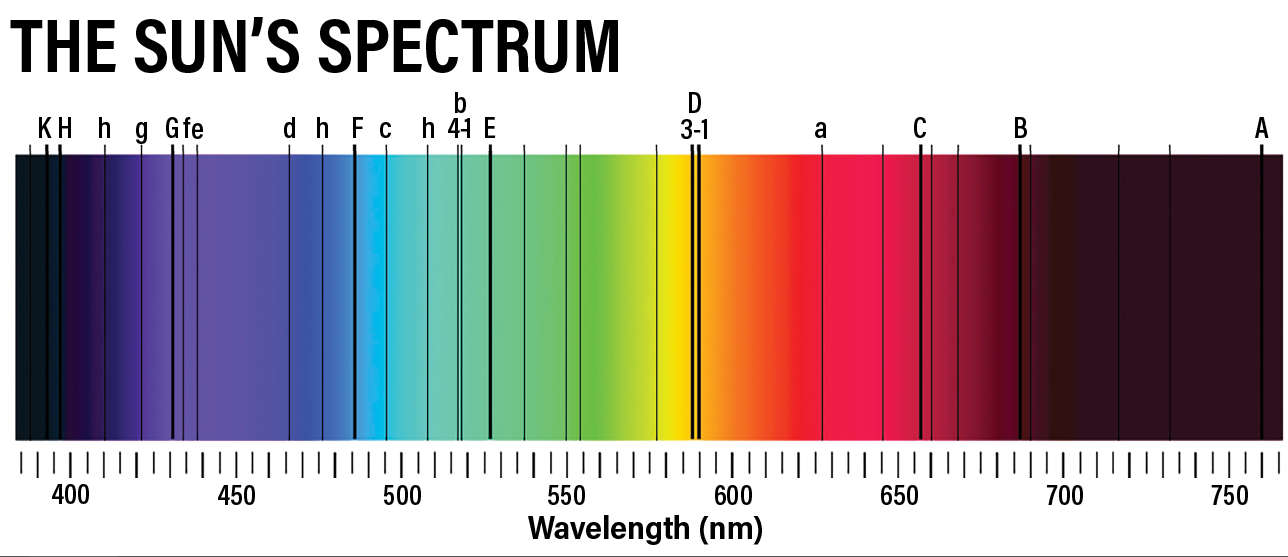
\includegraphics[scale = 0.25]{src/images/wavelengths.png}
        \caption{Wavelength (nm) and corresponding colors. Also shown are the Frauenhofer lines for the sun's spectrum.}
        \label{fig_wavelengths}
    \end{figure}

    \begin{figure}[H]
        \centering
        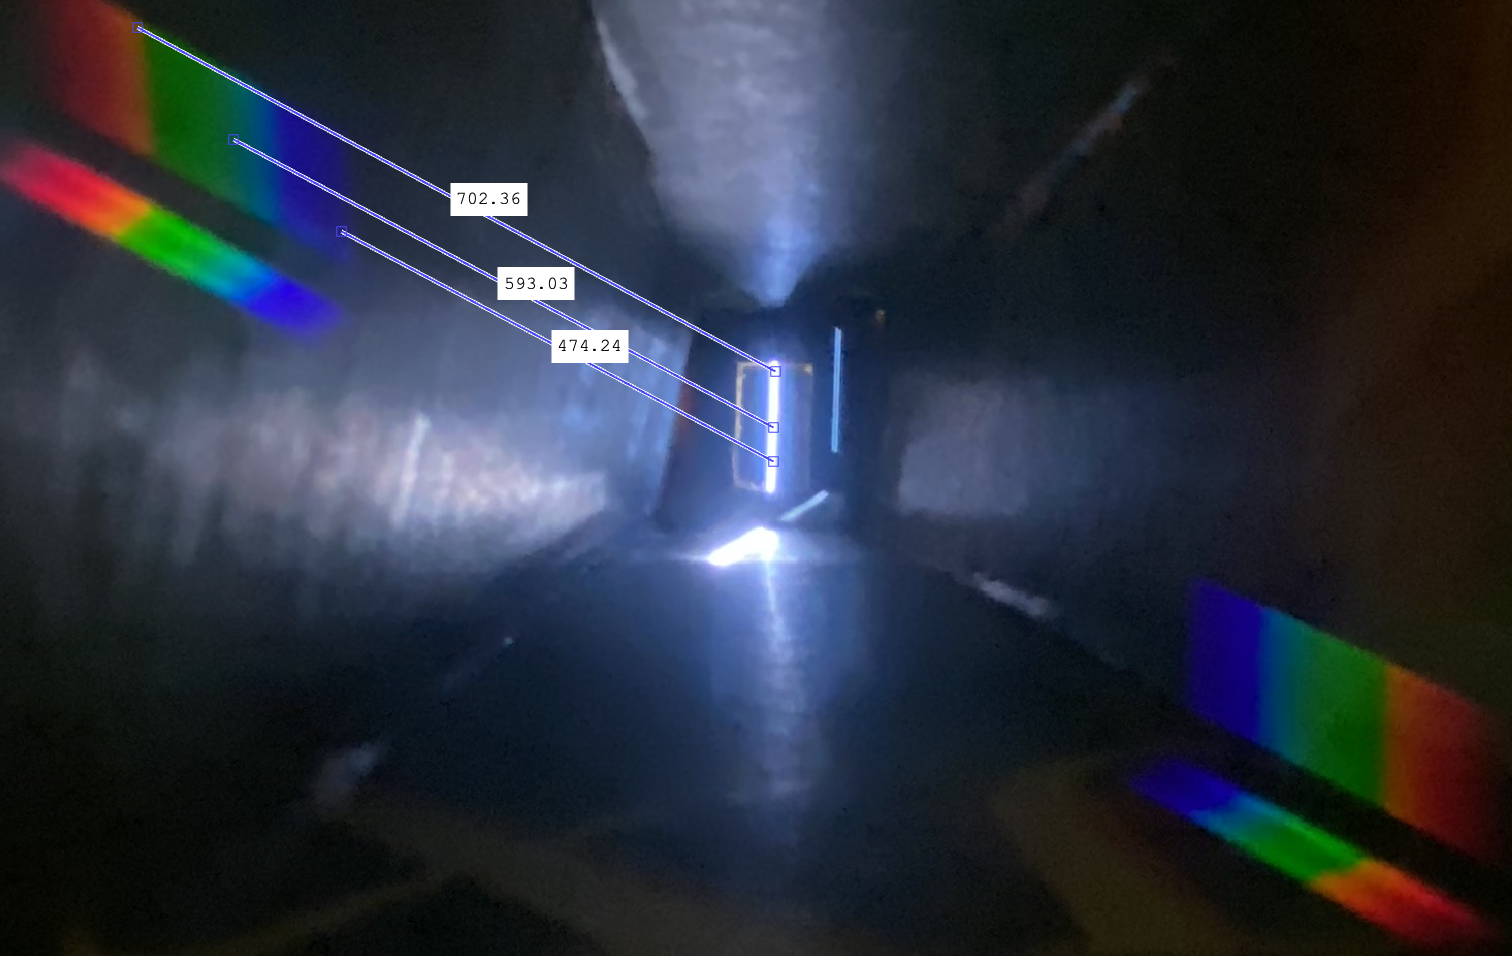
\includegraphics[scale = 0.39]{src/images/distance_calc.png}
        \caption{Spectrum of sunlight with measurements taken of certain points.}
        \label{fig_distance_calc}
    \end{figure}

    \begin{figure}[H]
        \centering
        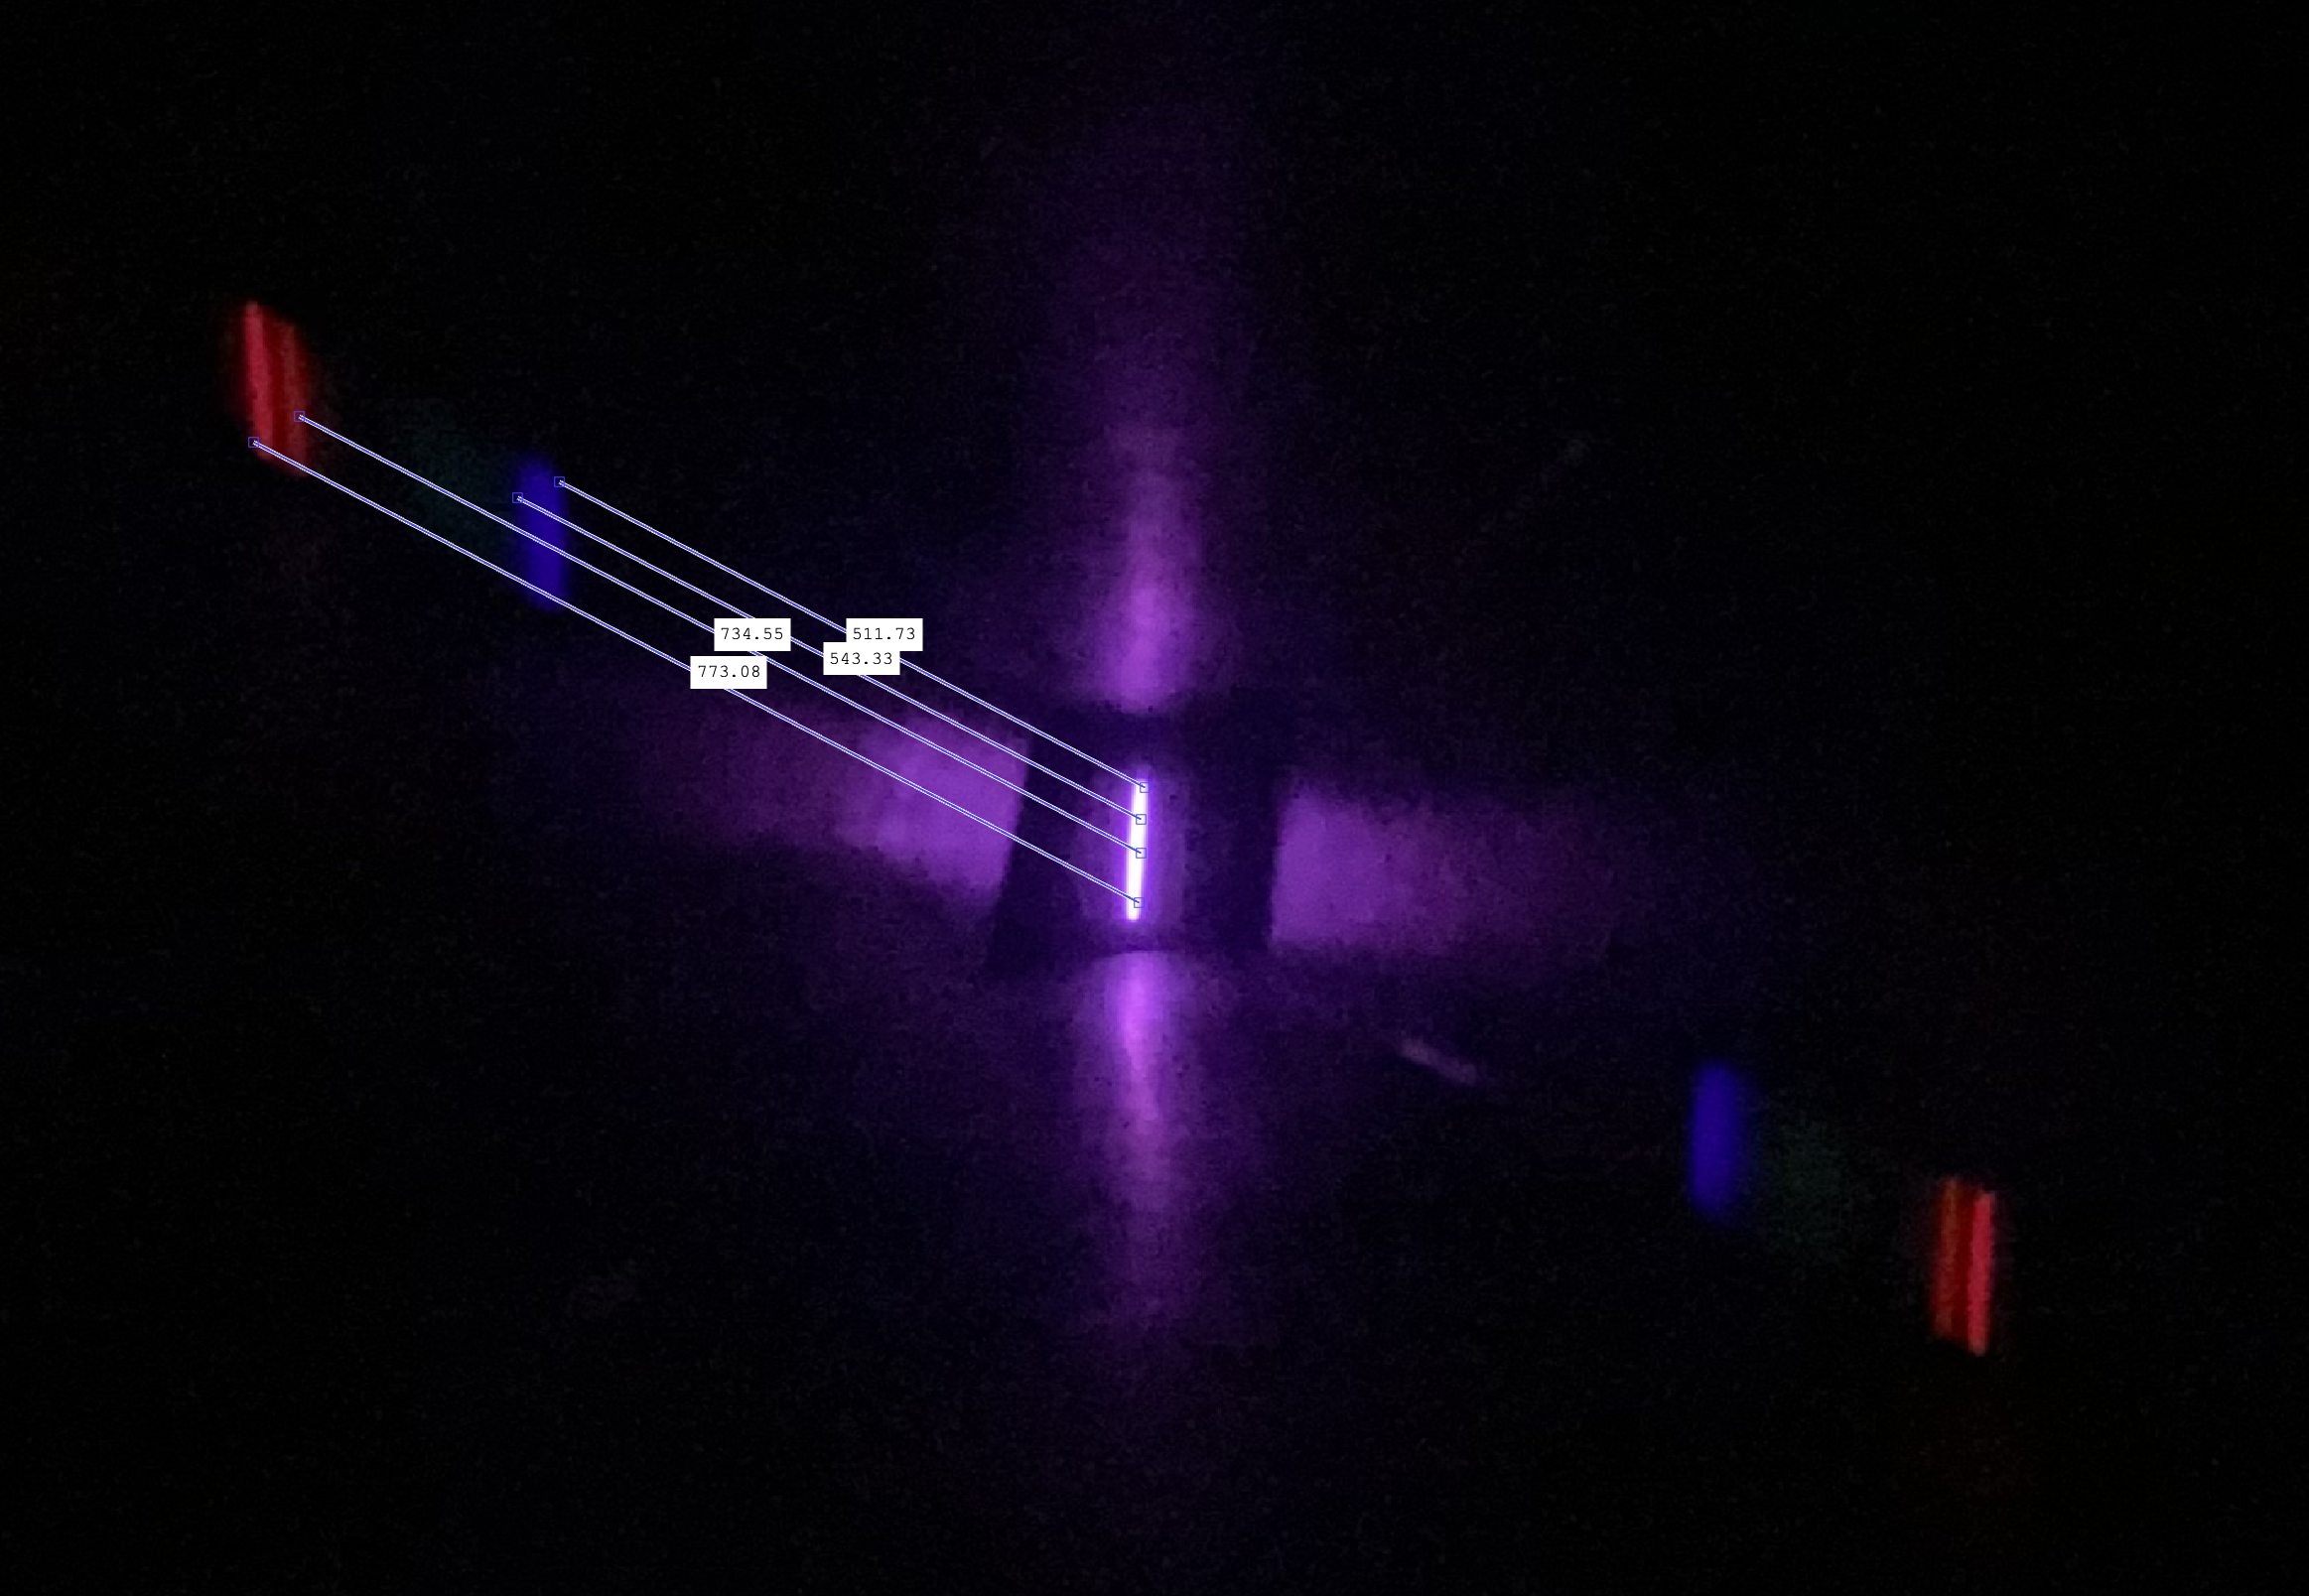
\includegraphics[scale = 0.25]{src/images/purple_screen_meas.png}
        \caption{Spectrum of a computer screen displaying a purple color.}
        \label{fig_purple_screen}
    \end{figure}

    \begin{figure}[H]
        \centering
        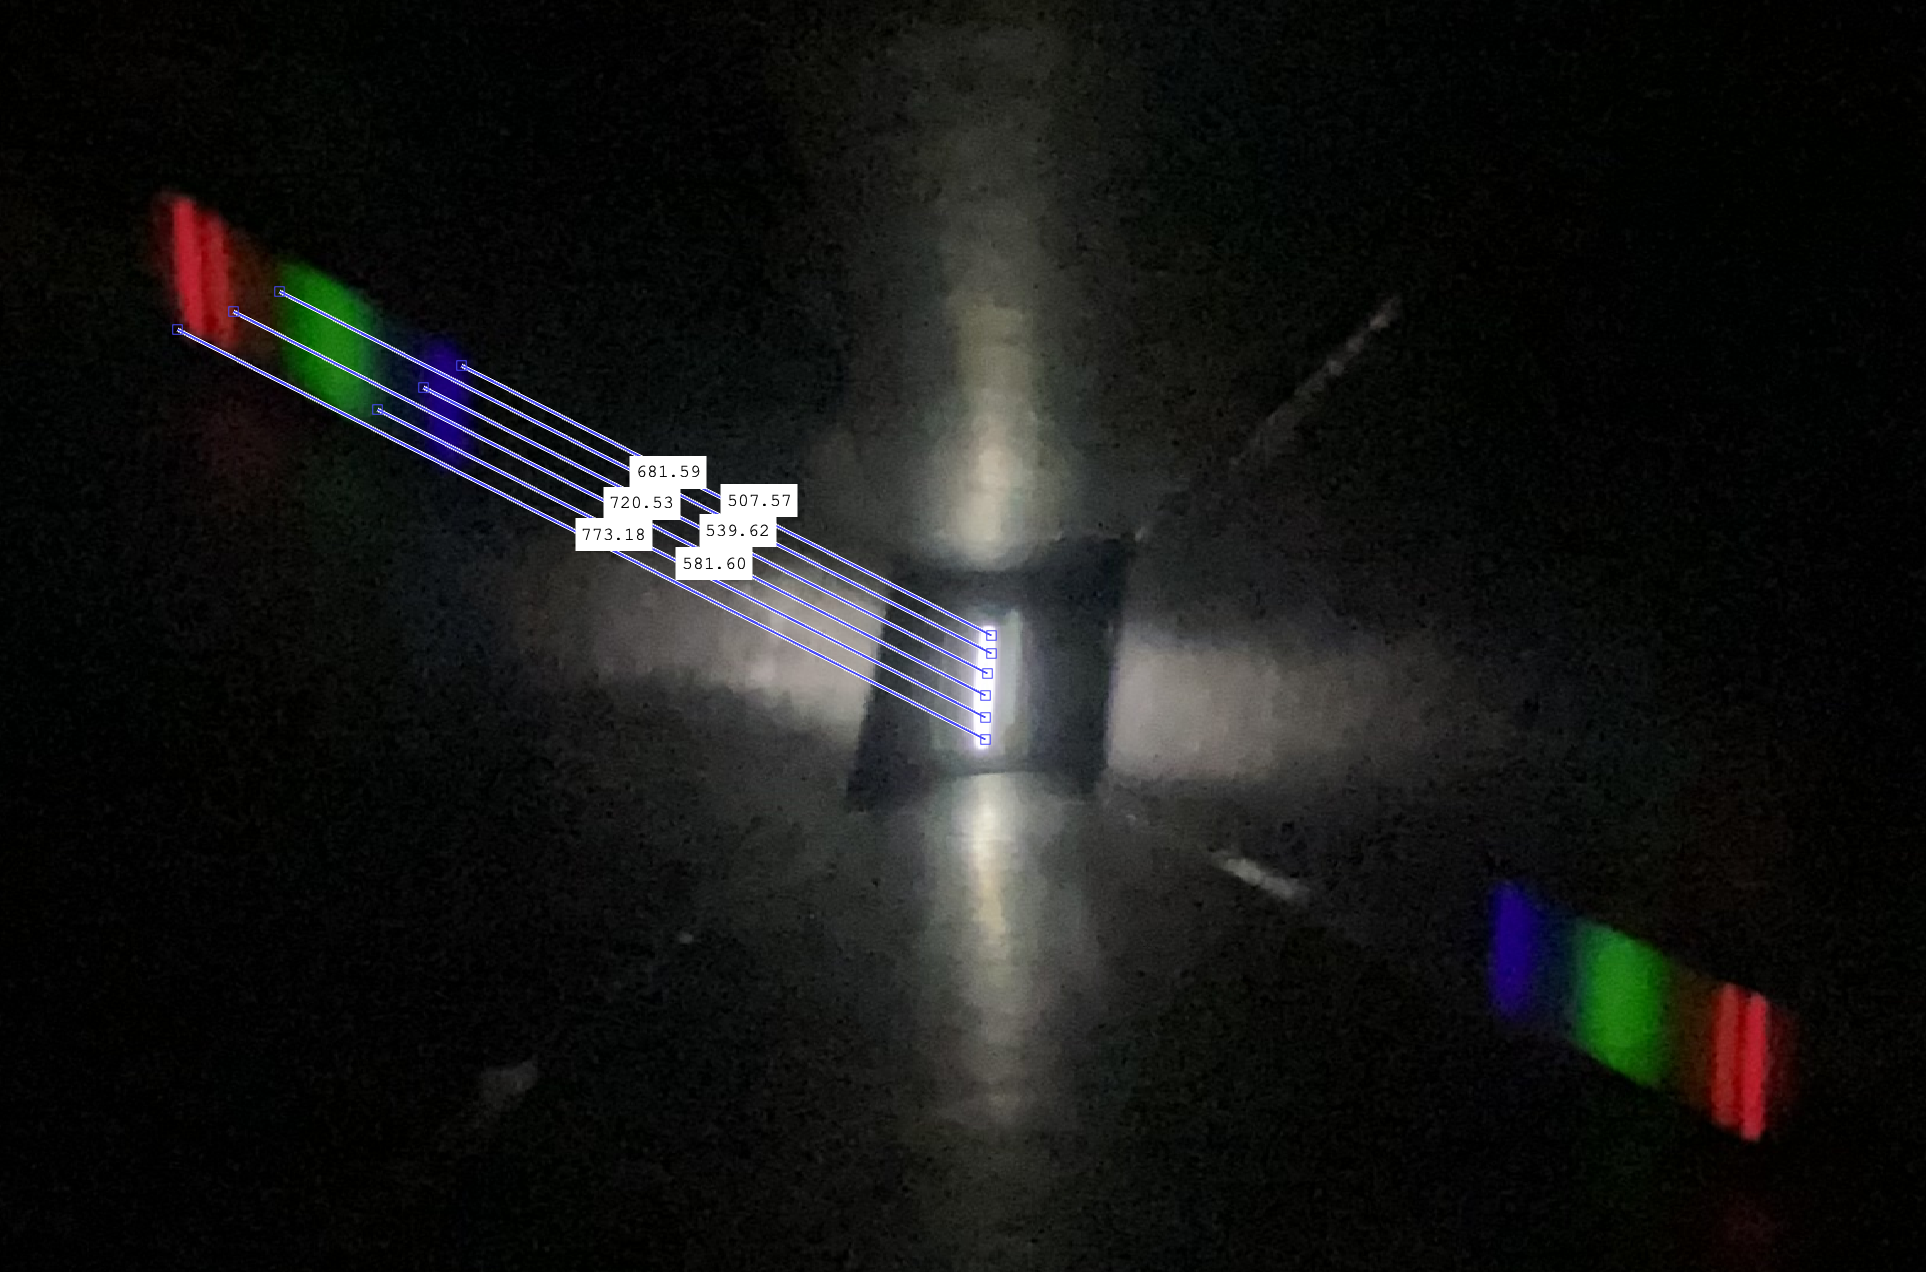
\includegraphics[scale = 0.31]{src/images/lamp1_meas.png}
        \caption{Spectrum of ceiling light. This light source only emits certain wavelengths.}
        \label{fig_lamp1}
    \end{figure}

    \begin{figure}[H]
        \centering
        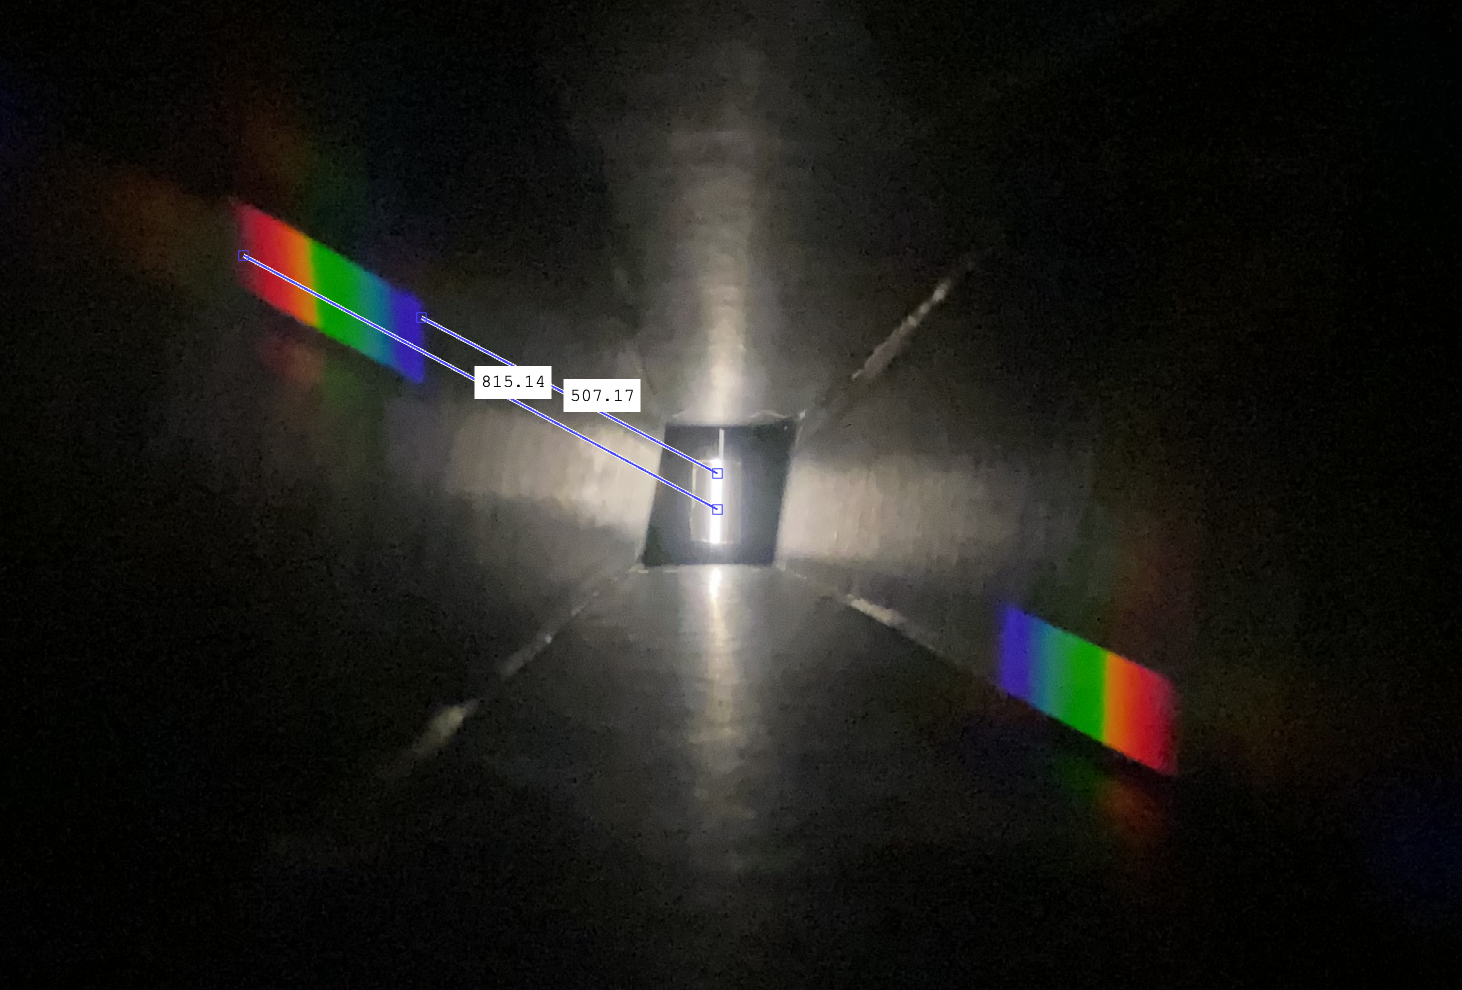
\includegraphics[scale = 0.41]{src/images/lamp2_meas.png}
        \caption{Spectrum of ceiling light. This light source emits almost the entire light spectrum.}
        \label{fig_lamp2}
    \end{figure}